% -----------------------------------------------------------------
% Document class: Article
\documentclass[ a4paper, twoside, 11pt]{article}
\usepackage{../../../macros-general}
\usepackage{../../../macros-article}
% Number of the handout, quiz, exam, etc.
\newcommand{\numero}{02}
\setcounter{numero}{\numero}

% -----------------------------------------------------------------
\begin{document}
\allowdisplaybreaks

\begin{center}
\Large Mec\'anica Vectorial (MECG-1001): Lecci\'on \numero \\[2ex]
\small \textbf{Semestre:} 2017-2018 T\'ermino II \qquad
\textbf{Instructor:} Luis I. Reyes Castro \qquad
\textbf{Paralelo:} 09
\end{center}
\fullskip

% =============================================
\begin{problem} Dos varillas de 500 mm est\'an conectadas mediante un pasador en $D$ como lo indica la figura de abajo, donde todas las dimensiones se muestran en milimetros. El punto $B$ se mueve hacia la izquierda con una velocidad constante de 360 mm/s. 

\begin{figure}[htb]
\centering
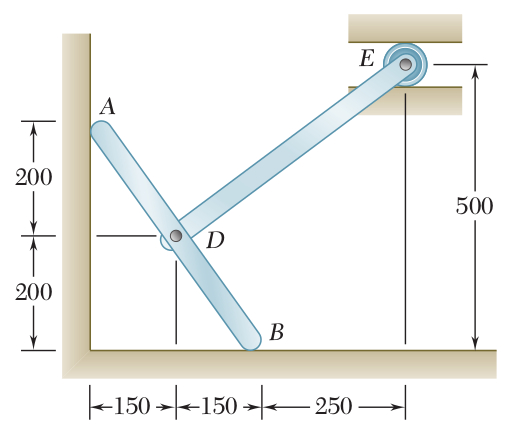
\includegraphics[width=0.46\textwidth]{problema-01.jpg}
\end{figure}

Complete las siguientes actividades: 
\begin{enumerate}[label=\textbf{\alph*)}]
\item \textbf{3 Puntos:} Encuentre la velocidad angular de la barra $AB$. \\[1ex] \emph{Soluci\'on:} Primero tomamos datos: 
\begin{align*}
\vec{v_B} \; & = \; ( \, -0.360, \, 0) \; \text{m/s} \\
\vec{v_A} \; & = \; ( \, 0, \, +v_A) \; \text{m/s} \\
\vec{v_E} \; & = \; ( \, +v_E, \, 0 ) \; \text{m/s} \\
\vec{r_{BA}} \; & = \; ( \, -0.300, \, +0.400 ) \; \text{m} \\
\vec{r_{BD}} \; & = \; ( \, -0.150, \, +0.200 ) \; \text{m} \\
\vec{r_{DE}} \; & = \; ( \, +0.400, \, +0.300 ) \; \text{m}
\end{align*}
Las velocidades en $A$ y $B$ est\'an relacionadas con la velocidad angular de la barra $AB$ de la siguiente manera:
\begin{align*}
& \vec{v_A} \; = \; \vec{v_B} + \vec{\omega_{AB}} \cross \vec{r_{BA}} \\
& \Longrightarrow \; \colvec{0}{+v_A} \; = \; 
\colvec{-0.360}{0} +
\colvec{ -0.400 \, \omega_{AB}}{ -0.300 \, \omega_{AB}} \\
& \Longrightarrow \;
0 \; = \; -0.360 - 0.400 \, \omega_{AB} \\
& \Longrightarrow \;
\vec{\omega_{AB}} \; = \; -0.75 \, \uvec{k} \; \text{rad/s}
\end{align*}
\item \textbf{2 Puntos:} Encuentre la velocidad en $D$. \\[1ex] \emph{Soluci\'on:} Las velocidades en $B$ y $D$ est\'an relacionadas con la velocidad angular de la barra $AB$ de la siguiente manera:
\begin{align*}
\vec{v_D} \; 
& = \; \vec{v_B} + \vec{\omega_{AB}} \cross \vec{r_{BD}} \\
& = \; \colvec{-0.360}{0} +
\colvec{ -0.200 \, (-0.75)}{ -0.150 \, (-0.75)} \\
& = \;
\colvec{ -0.21}{ +0.1125} \; \text{m/s} \; \equiv \;
0.2382 \; \text{m/s} \; \measuredangle 151.82\deg
\end{align*}
\item \textbf{3 Puntos:} Encuentre la velocidad angular de la barra $DE$. \\[1ex] \emph{Soluci\'on:} Las velocidades en $D$ y $E$ est\'an relacionadas con la velocidad angular de la barra $DE$ de la siguiente manera:
\begin{align*}
& \vec{v_E} \; = \; \vec{v_D} + \vec{\omega_{DE}} \cross \vec{r_{DE}} \\
& \Longrightarrow \; \colvec{+v_E}{0} \; = \; 
\colvec{-0.21}{+0.1125} +
\colvec{ -0.300 \, \omega_{DE}}{ +0.400 \, \omega_{DE}} \\
& \Longrightarrow \;
0 \; = \; +0.1125 + 0.400 \, \omega_{DE} \\
& \Longrightarrow \;
\vec{\omega_{DE}} \; = \; -0.281 \, \uvec{k} \; \text{rad/s}
\end{align*}
\item \textbf{2 Puntos:} Encuentre la velocidad en $E$. \\[1ex] \emph{Soluci\'on:} De la expresi\'on anterior tenemos: 
\begin{align*}
\vec{v_E} \;
& = \; \colvec{-0.21}{+0.1125} +
\colvec{ -0.300 \, (-0.281)}{ +0.400 \, (-0.281)} \\
& = \; \colvec{-0.1257}{0} \; \text{m/s} \; \equiv \;
0.1257 \; \text{m/s} \; \measuredangle \pm180\deg
\end{align*}
\end{enumerate}

\end{problem}
\fullskip

% =============================================
\begin{problem}
Tres barras, cada una con un peso de 8 lb, est\'an soldadas entre si y se encuentran conectadas mediante pasadores a los dos eslabones $BE$ y $CF$, los cuales tienen peso despreciable y longitud de 10 in. 

\begin{figure}[htb]
\centering
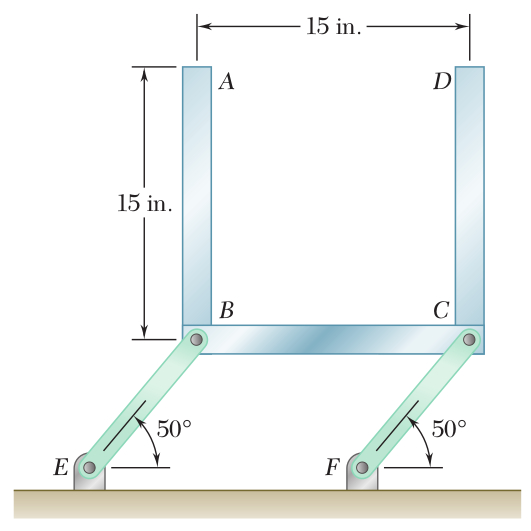
\includegraphics[width=0.46\textwidth]{problema-02.jpg}
\end{figure}

Complete las siguientes actividades: 
\begin{enumerate}[label=\textbf{\alph*)}]
\item \textbf{1 Punto:} Encuentre la locaci\'on del centro de masa del ensamble $ABCD$. \\[1ex] \emph{Soluci\'on:} Es evidente que como el ensamble es sim\'etrico entonces la coordenada $x$ de su centro de masa es igual a la coordenada $x$ del punto medio de la barra $BC$. Para hallar la coordenada $y$ definimos a $\delta$ como la distancia desde el punto medio de la barra $BC$ hasta el centro de masa del ensamble. Entonces tenemos:
\[
\delta \; = \; 
\frac{(8)(0.0) + 2(8)(7.5/12)}{3(8)} \; = \; 0.4167 \; \text{ft}
\]
\item \textbf{2 Puntos:} Encuentre la aceleraci\'on del centro de masa del ensamble $ABCD$ en funci\'on de la aceleraci\'on angular de la barra $BE$. 
\item \textbf{5 Puntos:} Determine la fuerza en cada eslab\'on inmediatamente despu\'es de que el sistema se suelta desde el reposo. 
\end{enumerate}

\end{problem}
\fullskip

% =============================================
\begin{problem}
\textbf{[6 Puntos]} Los extremos de una barra $AB$ de 9 lb est\'an restringidos a moverse a lo largo de ranuras cortadas en una placa vertical en la forma que se indica. Un resorte de constante $k = 3$ lb/in. se fija al extremo $A$ de manera tal que su tensi\'on es cero cuando $\theta = 0\deg$. La barra se suelta desde el reposo cuando $\theta = 50\deg$, determine la velocidad angular de la barra y la velocidad del extremo $B$ cuando $\theta = 0\deg$. 

\begin{figure}[htb]
\centering
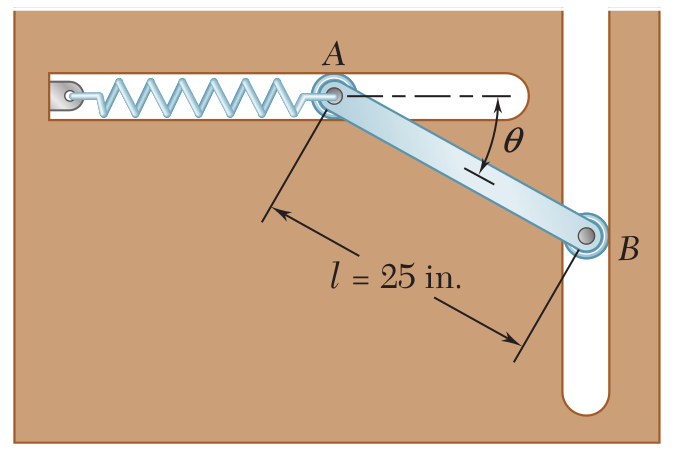
\includegraphics[width=0.5\textwidth]{problema-03.jpg}
\end{figure}

\end{problem}
\fullskip

\end{document}